\documentclass[times, utf8, zavrsni]{fer}
\usepackage{booktabs}
\usepackage{graphicx}
\usepackage{array}
\graphicspath{ {./img/} }

\begin{document}

% TODO: Navedite broj rada.
\thesisnumber{5417}

% TODO: Navedite naslov rada.
\title{Implementacija sustava za nadziranje i upravljanje bežičnim razvojnim modulima ESP8266}

% TODO: Navedite vaše ime i prezime.
\author{Ivan Trubić}

\maketitle

% Ispis stranice s napomenom o umetanju izvornika rada. Uklonite naredbu \izvornik ako želite izbaciti tu stranicu.
\izvornik

% Dodavanje zahvale ili prazne stranice. Ako ne želite dodati zahvalu, naredbu ostavite radi prazne stranice.
\zahvala{}

\tableofcontents

\chapter{Uvod}
ESP8266 je System on Chip (SoC) rješenje tvrtke Espresiff Systems vrlo malene površine mnogih mogučnosti.
Dizajniran je kao vrlo jeftin modul sa mogučnošću spajanja na WiFi mrežu te niskom potrošnjom energije što ga čini vrlo povoljnim za ugrađivanje u IoT (\textit{Internet Of Things}) uređaje.
U ovome će radu ESP8266 \textit{SoC} biti korišten kao krajnji čvor u sustavu bežičnog prikupljanja podataka, nadziranja te upravljanja koji komunicira s ostalim sustavom koristeći \textit{Message Queueing Telemetry Transport} protokol (MQTT).
Topologija takvog sustava se sastoji od krajnjeg čvora na kojem je spojen neki uređaj koji želimo kontrolirati ili nadzirati, pristupne točke WiFi mreži, poslužitelja na kojemu se nalaze MQTT broker za upravljanje porukama, baza podataka koja sadrži trenutne podatke čvorova te API kao sučelje između baze podataka i krajnjeg klijenta.
Ovakav sustav je vrlo jednostavan i jeftin za implementaciju te je izrazito jako skalibilan što znači da pisanjem vrlo jednostavnog programskog koda za pojedini čvor možemo u svoju mrežu postaviti virtualno beskonačno krajnjih čvorova kojima se vrlo jednostavno može upravljati. 
Cilj ovoga rada je napraviti gotov sustav otvorenoga koda koji će prateći \textit{Homie} konvenciju za MQTT protokol olakšati amaterima brzo rađenje prototipa bilo iz znatiželje, potrebe ili kreativnosti.

\chapter{Razrada}

\section{ESP8266}
ESP8266 je \textit{SoC} koji u sebi ima mikrokontroler RISC arhitekture te WiFi modul za spajanje na mrežu.
Ciljano tržište za ovaj čip su hobisti koji žele neku svoju ideju pretvoriti u stvarnost na vrlo jednostavan način.
Dizajniran je vrlo jednostavno i kompaktno kako bi cijena čipa bila što niža te zato što je namjenjen za jednostavne i lokalizirane poslove koji uključuju upravljanje vrlo malim brojem uređaja odjednom.
Točno u tome leži prava snaga čipa jer možemo imati više čipova koji komuniciraju međusobno umjesto da imamo jedan snažan mikrokontroler koji će upravljati uređajima centralizirano.

\begin{figure}[h]
    \centering
    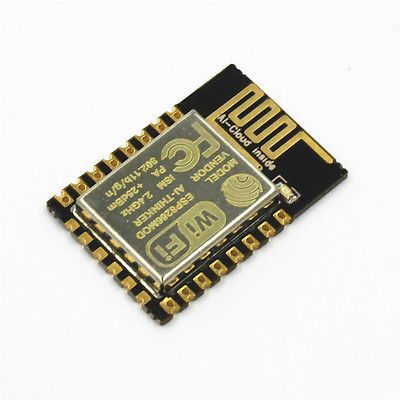
\includegraphics[scale=0.5]{esp8266.jpg}
    \caption{ESP8266 \textit{SoC}}
\end{figure}

\section{Značajke}
ESP8266 u sebi ima 32-bitni RISC mikrokontroler koji radi na frekvenciji od 80MHz.
Memorija se sastoji od:
\begin{itemize}
    \item 32 KiB instrukcijskog RAM-a
    \item 32 KiB priručne memorije instrukcijskog RAM-a
    \item 80 KiB korisničkog RAM-a
\end{itemize}
Vanjske QSPI \textit{flash} memorije do 16MiB ovisno o modelu, IEEE 802.11 b/g/n WiFi, 16 GPIO pina, SPI sučelje, softverska implementacija I2C protokola, I2S sučelje, UART te 10-bitni analogno-digitalni pretvornik.


\section{Povezivost}
Najbitnije sučelje prema vanjskome svijetu na ESP8266 su bežična mreža i 16 GPIO pinova.
Mreža podržava IEEE 802.11 b/g/n protokol, P2P konfiguraciju te TCP/IP protokolni stog.
GPIO pinovi se mogu zasebno programirati kao ulazi/izlazi, postaviti im \textit{pull-up/down} otpornike, te svaki ima ugrađen 10 bitni digitalno-analogni pretvornik tako da se svaki pin ponaša kao analogni izlaz.
Ima također jedan analogan ulaz sa 10 bitnim analogno-digitalnim pretvornikom za spajanje raznih analognih senzora bez posebnih sučelja.

\section{Programiranje}
ESP8266 se može programirati na više različitih načina.
Originalno se programirao uz pomoć drugoga mikrokontrolera sve dok firma Espressif Systems nije izdala poseban \textit{SDK}(  eng. \textit{Software Development Kit} ) nakon čega to više nije bilo potrebno.
Nakon toga su se počeli javljat mnogi SDK-ovi ponajviše otvorenog koda zajednice programera od čega su najpoznatiji:
    \begin{itemize}
        \item NodeMCU - baziran na skriptnom programskom jeziku Lua
        \item Arduino - baziran na jeziku C++ iste sintakse kao i bilokoji arduino mikrokontroler
        \item PlatformIO - nova razina razvoja ugradbenih sustava sa posebnim IDE-om
        \item MicroPython - baziran na programskom jeziku python
    \end{itemize}

\section{Usporedba drugih razvojnih modula koji koriste WiFi komunikacijski protokol sa ESP8266 modulom}
Usporedba raznih arduina i slicnih mikrokontrolera koji se mogu spojiti na WiFi.

\begin{center}
    \begin{tabular}{ |c|c|c|c|c| }
        \hline
        \textbf{naslov} & \textbf{naslov} & \textbf{naslov} & \textbf{naslov} & \textbf{naslov} \\
        \hline
        cell1 & cell2 & cell3 & cell 4 & cell5\\
        \hline
        cell6 & cell7 & cell8 & cell9 & cell10 \\
        \hline
    \end{tabular}
\end{center}

\section{Message Queuing Telemetry Transport - \textbf{MQTT}}
MQTT je protokol široko primjenjen u \textit{IoT} sustavima temeljen na prijenosu poruka u režimu pretplate i objave.
Prijenos poruka se vrši preko TCP/IP protokola te se za to brine program na poslužitelju koji ima ulogu brokera.

\section{Homie konvencija za MQTT protokol}

\chapter{Programska podrška za praćenje komunikacije više modula ESP8266 na WiFi mreži}
\section{Implementacija MQTT klijenta na ESP8266 pomoću Homie konvencije}
\section{Postavljanje poslužitelja}
\section{Parser}
\section{API}

\chapter{Zaključak}
Zaključak.

\bibliography{literatura}
\bibliographystyle{fer}

\begin{sazetak}
Sažetak na hrvatskom jeziku.

\kljucnerijeci{Ključne riječi, odvojene zarezima.}
\end{sazetak}

% TODO: Navedite naslov na engleskom jeziku.
\engtitle{Management Framework for ESP8266 WiFi Development Modules}
\begin{abstract}
Abstract.

\keywords{Keywords.}
\end{abstract}

\end{document}
